\documentclass[11pt]{article}

\usepackage{amsmath}
\usepackage{amssymb}
\usepackage{graphicx}
\usepackage{caption}
\usepackage{subcaption}

\newcommand{\code}[1]{\texttt{#1}}

\begin{document}

\author{Gu, Qiao}
\title{16-720B Homework 1 Write-up}
\maketitle

\medskip

\subsection*{Q1.1.1}

\textbf{Gaussian filters} can smooth images and thus remove noise and details. Therefore, they can capture the ``averaged'' intensity of images over a scale.

\textbf{Laplacian of Gaussian} yields high responses at points where there are rapid changes in intensity. Specifically, Laplacian of Gaussian can capture peaks of intensity.

\textbf{Derivatives of Gaussian in x/y direction} gives high responses at edges in x and y direction repectively, and thus they capture the edge information of images.

\textbf{Multiple scales} are needed because the information mentioned above can happen at any scale, and multiple filters of different scales can capture them in different scales.

\newpage

\subsection*{Q1.1.2}

Please see the Figure~\ref{fig:q1.1.2} for the filter responses

\begin{figure}[h!]
    \centering
    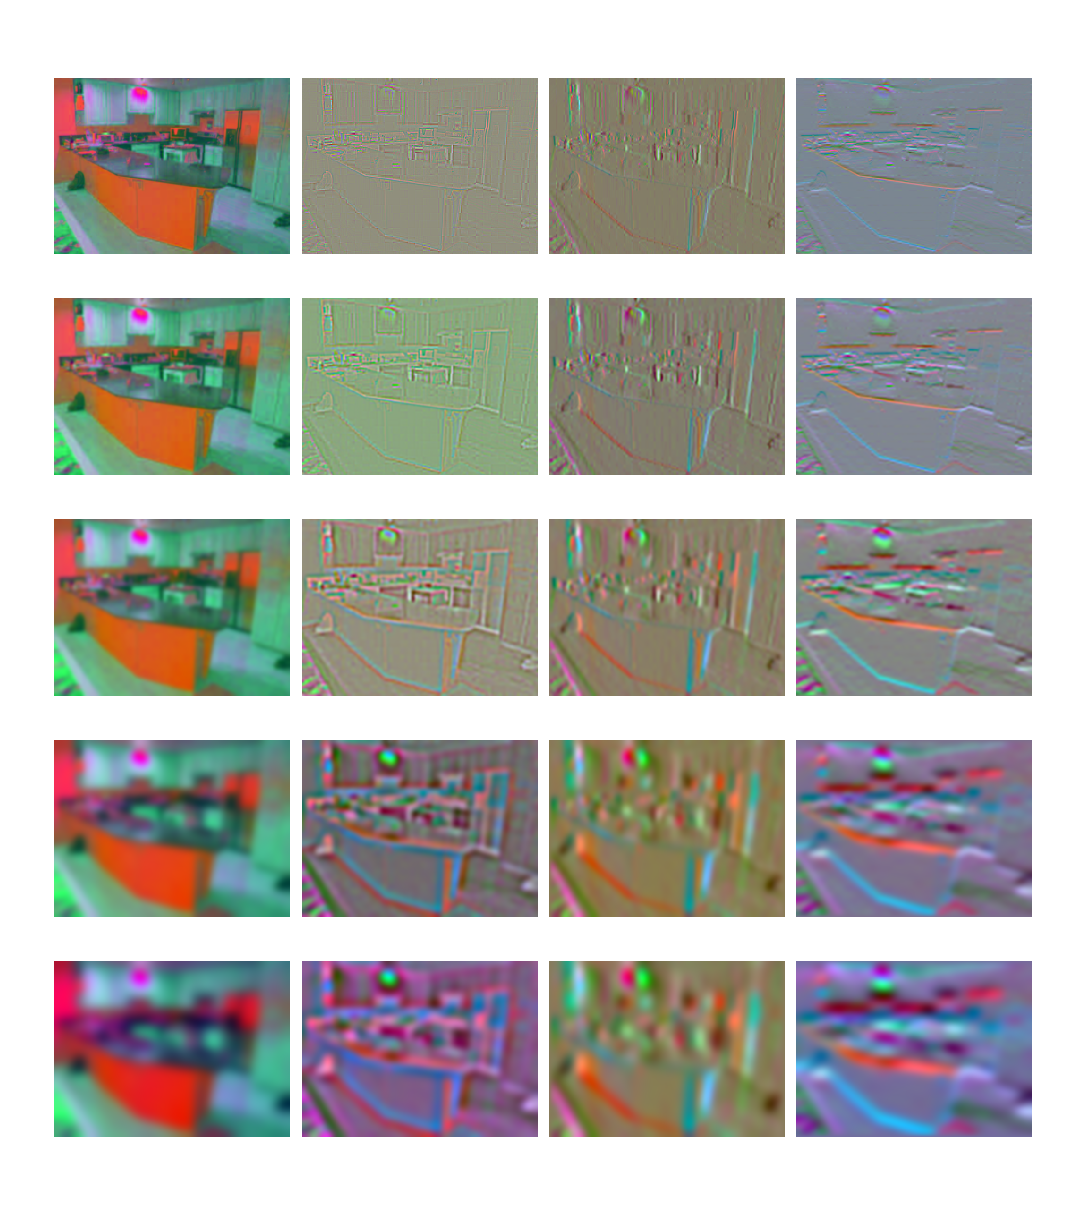
\includegraphics[width=\linewidth]{../results/q1_1_2_responses.png}
    \caption{Filter responses on the image \code{aquarium/sun\_aztvjgubyrgvirup.jpg}.}
    \label{fig:q1.1.2}
\end{figure}

\newpage

\subsection*{Q1.3}

Please see the Figure.~\ref{fig:q1.3} for the images and their wordmaps.

Yes these wordmaps indeed make sense to me. We can see that within one object, the color tends to be the same, which reflects the homogeneous texture of its appearance captured by Gaussian filters. When it goes to the boundary, there are one or more color strips on the borderline, and this reflects the different types of edges captured by derivatives and Laplacian of Gaussian filters.

\begin{figure}[h!]
  \center
  \begin{subfigure}{0.4\linewidth}
    \centering
    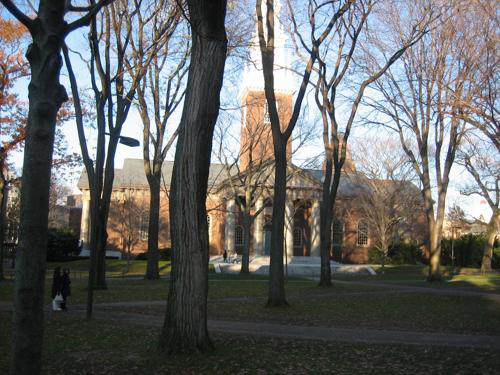
\includegraphics[width=\textwidth]{../results/labelme_brrdxeoavpkqjzs_image.png}
  \end{subfigure}
  \begin{subfigure}{0.4\linewidth}
    \centering
    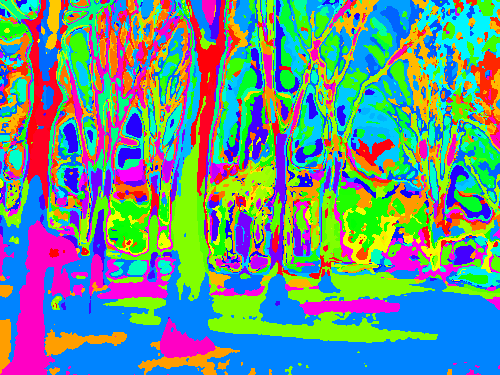
\includegraphics[width=\textwidth]{../results/labelme_brrdxeoavpkqjzs_wordmap.png}
  \end{subfigure}

  \begin{subfigure}{0.4\linewidth}
    \centering
    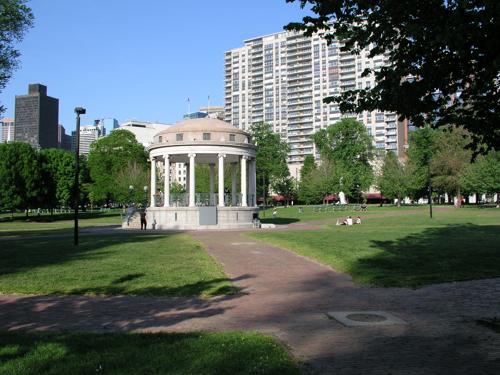
\includegraphics[width=\textwidth]{../results/labelme_caqoztrngzoasnb_image.png}
  \end{subfigure}
  \begin{subfigure}{0.4\linewidth}
    \centering
    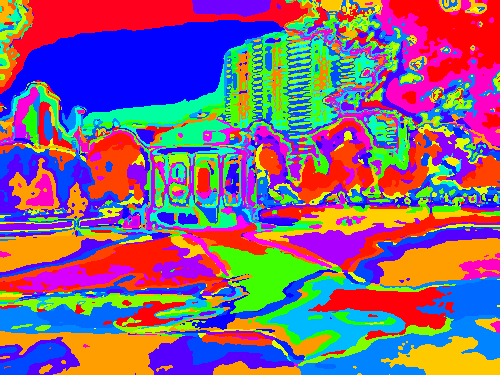
\includegraphics[width=\textwidth]{../results/labelme_caqoztrngzoasnb_wordmap.png}
  \end{subfigure}

  \begin{subfigure}{0.4\linewidth}
    \centering
    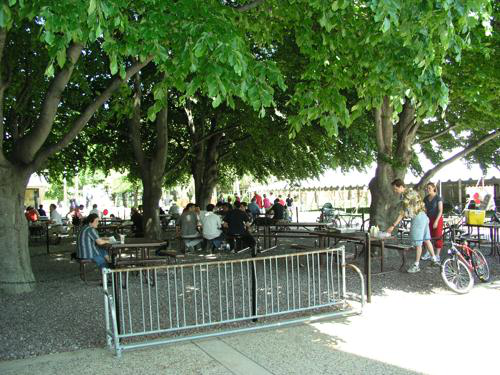
\includegraphics[width=\textwidth]{../results/labelme_zbyarunxxqdfebc_image.png}
  \end{subfigure}
  \begin{subfigure}{0.4\linewidth}
    \centering
    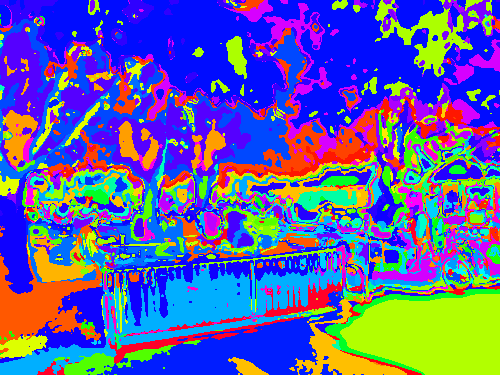
\includegraphics[width=\textwidth]{../results/labelme_zbyarunxxqdfebc_wordmap.png}
  \end{subfigure}

  \caption{Images and their wordmaps. }
  \label{fig:q1.3}
\end{figure}

\newpage

\subsection*{Q2.5}

The overall accuracy is $0.64375$, and the confusion matrix is as follows:

\begin{verbatim}
  [[14.  0.  0.  0.  0.  0.  0.  0.]
   [ 0. 14.  0.  1.  0.  1.  2.  0.]
   [ 0.  0. 15.  4.  3.  0.  0.  3.]
   [ 1.  2.  1. 17.  0.  0.  1.  4.]
   [ 1.  1.  0.  0. 10.  1.  0.  0.]
   [ 0.  2.  0.  1.  8. 12.  1.  0.]
   [ 0.  5.  0.  0.  2.  3. 11.  0.]
   [ 0.  2.  3.  2.  1.  1.  0. 10.]]
\end{verbatim}

\newpage

\subsection*{Q2.6}



% Failure cases: (path, label, predicted_label)
% ('kitchen/sun_aydvvhqombqloffb.jpg', 4, 0)
% ('kitchen/sun_aegnmfnvbbzeqjus.jpg', 4, 5)
% ('kitchen/sun_aueoksosdjqlckgv.jpg', 4, 1)
% ('waterfall/sun_aybtbiqdtgfuqbza.jpg', 6, 5)
% ('waterfall/sun_bcfzpnfpngukrlki.jpg', 6, 5)
% ('highway/sun_byinrjsphbeujidj.jpg', 3, 0)
% ('highway/sun_brhayiyxozkhqnug.jpg', 3, 1)
% ('highway/sun_bhdcdduciijbbnss.jpg', 3, 1)
% ('highway/sun_bnvkyxyoayuaccah.jpg', 3, 2)
% ('highway/sun_buaguirojqkqtzdv.jpg', 3, 6)
% ('highway/sun_bosmbhpldtmjdgxs.jpg', 3, 7)
% ('highway/sun_bsqoowlelpxyjkyt.jpg', 3, 7)
% ('highway/sun_bnxsatkjkhtpezcd.jpg', 3, 7)
% ('highway/sun_bgeixfvonqvlpwhg.jpg', 3, 7)
% ('waterfall/sun_bximgaxujsdbqunl.jpg', 6, 1)
% ('waterfall/sun_bnztrbwcwwkkrnum.jpg', 6, 1)
% ('waterfall/sun_aelikoqdertbwulp.jpg', 6, 1)
% ('waterfall/sun_bhczjtvnuhhqeaxg.jpg', 6, 1)
% ('waterfall/sun_browhtghljbzuemv.jpg', 6, 1)
% ('waterfall/sun_algsdnkyqawwgfol.jpg', 6, 4)
% ('waterfall/sun_amlayefazeitmzuj.jpg', 6, 4)
% ('waterfall/sun_aszeweschfcslhif.jpg', 6, 5)
% ('park/labelme_zktlrcrhggzuszr.jpg', 1, 5)
% ('park/labelme_tmaidzxwwhxhtor.jpg', 1, 6)
% ('park/labelme_xuntpkgfijknxde.jpg', 1, 3)
% ('park/labelme_xudibcwieqslwxd.jpg', 1, 6)
% ('desert/sun_bqxjwczwiwnzkrbj.jpg', 2, 3)
% ('desert/sun_bqujpdxcuslyzejj.jpg', 2, 3)
% ('desert/sun_bytguqqbadccqkyt.jpg', 2, 3)
% ('desert/sun_bgwdwaeuakbmuxeg.jpg', 2, 3)
% ('desert/sun_biozxhxgtfrmoagh.jpg', 2, 4)
% ('desert/sun_banypouestzeimab.jpg', 2, 4)
% ('desert/sun_bcmhdbzhuexunnaq.jpg', 2, 4)
% ('desert/sun_brvgfhfxhmxhmpps.jpg', 2, 7)
% ('desert/sun_ajrputhzcjawjvzm.jpg', 2, 7)
% ('desert/sun_bdcttfhebcktjrep.jpg', 2, 7)
% ('windmill/sun_bcyuphldelrgtuwd.jpg', 7, 1)
% ('windmill/sun_beqradarsjammmwv.jpg', 7, 1)
% ('windmill/sun_arzqgolrrmfeptxe.jpg', 7, 2)
% ('windmill/sun_bidwiikkuntuvlkz.jpg', 7, 2)
% ('windmill/sun_belpgdpjevtjgyfv.jpg', 7, 2)
% ('windmill/sun_bxzsglbilsxviyio.jpg', 7, 3)
% ('windmill/sun_avgtzbktnevdkgsy.jpg', 7, 3)
% ('windmill/sun_bdemofubbftpwgaz.jpg', 7, 4)
% ('windmill/sun_bymqbzsknamqhokg.jpg', 7, 5)
% ('laundromat/sun_adwdzlyupqmkmvqj.jpg', 5, 1)
% ('laundromat/sun_addinpsdbmiewyvc.jpg', 5, 1)
% ('laundromat/sun_ambnszkijszxfzqj.jpg', 5, 3)
% ('laundromat/sun_aiewbfesvvdzrhei.jpg', 5, 4)
% ('laundromat/sun_asesjaotzrbpqdbk.jpg', 5, 4)
% ('laundromat/sun_afcrlioyduvyuqov.jpg', 5, 4)
% ('laundromat/sun_axwfgbwbszyyahzc.jpg', 5, 4)
% ('laundromat/sun_ahiqevcbekkuiqhb.jpg', 5, 4)
% ('laundromat/sun_awytptirbthbwszg.jpg', 5, 4)
% ('laundromat/sun_ayzamcvuelghoqrr.jpg', 5, 4)
% ('laundromat/sun_aaxufyiupegixznm.jpg', 5, 4)
% ('laundromat/sun_aeyuobflqlynijyl.jpg', 5, 6)

\newpage

\subsection*{Q3.2}

The overall accuracy is $0.975$, and the confusion matrix is as follows:

\begin{verbatim}
  [[14.  0.  0.  0.  0.  0.  0.  0.]
   [ 0. 17.  0.  0.  0.  0.  0.  1.]
   [ 0.  0. 24.  0.  0.  0.  0.  1.]
   [ 0.  0.  0. 26.  0.  0.  0.  0.]
   [ 0.  0.  0.  0. 12.  1.  0.  0.]
   [ 0.  0.  0.  0.  1. 23.  0.  0.]
   [ 0.  0.  0.  0.  0.  0. 21.  0.]
   [ 0.  0.  0.  0.  0.  0.  0. 19.]]
\end{verbatim}

We can see that the result accuracy and confusion matrix are much better than the those given by the classical BoW. I believe this is because since deep neural network (DNN) has deeper structure of convolutional layers, it has a much stronger capability of capturing high-level feature: DNN can synthesize the filter responses from different positions using another structured filter ratherthan simply calculate the histogram of filter responses of different scales and locations.

\end{document}
